\documentclass[11pt]{article}


%%%%%%%%%%%%%%%%5
\usepackage[utf8]{inputenc}
\usepackage{polski}
\usepackage{graphicx}
\usepackage{mathtools}
\usepackage{amsmath}
\usepackage{algorithm,algorithmic}
\usepackage[section]{placeins}
\usepackage{titlesec}
\usepackage{interval}
\usepackage[table]{xcolor}
\titlelabel{\thetitle.\quad}
\usepackage{caption}
\usepackage{subfig}



\topmargin=-0.45in
\evensidemargin=0in
\oddsidemargin=0in
\textwidth=6.5in
\textheight=9.0in
\headsep=0.25in

\linespread{1.1} % Line spacing


%%%%%%%%%%%%%%%%%

\date{Wrocław, \today}
\title{\LARGE\textbf{Analiza Numeryczna (M) - Pracownia 2 - Zadanie P2.10}\\Aproksymacja średniokwadratowa dyskretna\\ \normalsize{Prowadzący: dr hab. Paweł Woźny}}
\author{Karolina Jeziorska}
        
\begin{document}
\maketitle



\thispagestyle{empty}     
\tableofcontents   

\section{Wstęp}
Aproksymacja dyskretna, a dokładniej aproksymacja jaka pojawiła się w zadaniu (na zaburzonych danych) jest ściśle związana z analizą danych  eksperymentalnych. Badając zjawiska fizyczne, przyrodnicze, ekonomiczne itp... uzyskujemy konkretne wartości. Jednak w celu ogólniejszej interpretacji należy opisać te dane jakąś zależnością, funkcją. Wydaje się, że odpowiedzią na ten problem jest interpolacja, co jednak jest dość mylące. Interpolacja przechodzi przez podane węzły, ale między nimi może zachowywać się niekontrolowanie, szczególnie jeśli mamy dużo węzłów. Dodatkowo, nasze wartości zwykle nie są dokładne, pomiary zazwyczaj obarczone są błędem. Dlatego nie zależy nam, by funkcja opisująca dane przechodziła dokładnie przez nie. Widać, że jednak lepszym rozwiązaniem problemu jest aproksymacja, która zminimalizuje sumaryczny błąd, czyli przybliży nas do pierwotnej funkcji jaką opisywały dane. W tym sprawozdaniu opiszę aproksymację średniokwadratową dyskretną.

\section{Teoretyczne omówienie problemu}
\subsection{Zadanie aproksymacji}
Klasyczne zadanie aproksymacji możemy zdefiniować następująco: dla danej funckji $f$ spośród funkcji ustalonej klasy poszukujemy tej funkcji $g$, która w określonym sensie najlepiej przybliża $f$. Sens tej najlepszej aproksymacji zależy od wyboru normy.

\subsection{Aproksymacja średniokwadratiowa dyskretna}
Powyższa definicja przy rozwiązywaniu zadania aproksymacji sprowadza się do rozwiązania zadania: szukamy takiego $w_n \in \Pi_n$ (gdzie $\Pi_n$ to wszystkie wielomiany stopnia niewiększego niż $n$), że dla każdego $w \in \Pi_n$ zachodzi:

\begin{equation*}
||f - w_n || < ||f - w||
\end{equation*}

Co jest równoważne stwierdzeniu:
\begin{equation*}
||f - w_n || = \inf_{w \in \Pi_n} ||f - w||
\end{equation*}

W aproksymacji średniokwadratowej dyskretnej nie mamy podanej funkcji $f$ tylko jej wartosci w skończonej liczbie punktów (przyjmijmy, że mamy m punktów). Dlatego też $||f - w_n ||$ wyraża się wzorem:
\begin{equation}
\sum_{i=0}^m p(x_i) \Big[f(x_i) - w_n(x_i)\Big]^2
\label{wzor:wzor1}
\end{equation}
Gdzie iloczyn skalarny to:
\begin{equation}
<f,g> = \sum_{i=0}^m p(x_i) f(x_i) g(x_i)
\label{wzor:wzor2}
\end{equation}

Należy zwrócić też uwagę na $p(x)$ czyli funkcję wagową. Określa dokładność aproksymacji w danym punkcie. Jako, że w rozważanym zadaniu wszystkie punkty są jednakowo ważne, to $p(x) = 1$.

\subsection{Rozwiązanie problemu aproksymacji}
Wielomian $w_n$ możemy przedstawić jako kombinację liniową wielomianów bazowych $P_i$: 
\begin{equation*}
w_n = \sum_{j = 0}^n a_i P_i
\end{equation*}
Po podstawieniu do wzoru \ref{wzor:wzor1} dostajemy:
\begin{equation}
||f - w_n|| = \sum_{i=0}^m p(x_i) \Big[f(x_i) - \sum_{j = 0}^n a_i P_i\Big]^2 = D(a_0, a_1, \dots , a_n) 
\end{equation}

Mamy funkcję $n+1$ zmiennych i szukamy jej minimum, czyli dla każdego $a_k$ $(k = 0,1, \dots , n)$ liczymy pochodną i przyrównujemy ją do $0$:

\begin{align*}
\frac{\partial D}{\partial a_k} &= 0 \\
-2 \sum_{i=0}^m p(x_i) \Big[f(x_i) - \sum_{j = 0}^n a_i P_i\Big]P_k(x_i) &= 0\\
\sum_{i=0}^m p(x_i)f(x_i)P_k(x_i) &= \sum_{i=0}^m p(x_i)P_k(x_i) \sum_{j = 0}^n a_j P_j(x_i)\\
<f,P_k> &= \sum_{j = 0}^n a_j \sum_{i=0}^m p(x_i)P_k(x_i)P_j(x_i) \\
<f,P_k> &= \sum_{j = 0}^n a_j <P_k, P_j>
\end{align*}

Biorąc wszystkie równania możemy układ przedstawić w postaci macierzowej:
\begin{equation}
\begin{bmatrix}
<P_0,P_0> & <P_0,P_1> & \hdots & <P_0,P_n>\\
<P_1,P_0> & <P_1,P_1> & \hdots & <P_1,P_n>\\
\vdots &  &  & \vdots\\
<P_n,P_0> & <P_n,P_1> & \hdots & <P_n,P_n>\\
\end{bmatrix}
\begin{bmatrix}
\alpha_0 \\
\alpha_1 \\
\vdots \\
\alpha_n
\end{bmatrix} = 
\begin{bmatrix}
<f,P_0>\\
<f,P_1>\\
\vdots \\
<f,P_n>
\end{bmatrix}
\end{equation}

Mamy n+1 równań i n+1 niewiadomych. Dla dużych $n$ liczenie rozwiązania może być skomplikowane i czasochłonne - o ile układ ma jednoznaczne rozwiązanie.
  
Jak spojrzymy na podany układ to łatwo zauważyć, że rozwiązanie będzie oczywiste i jednoznaczne, gdy macierz iloczynów skalarnych funkcji bazowych poza przekątną będzie miała wartości zerowe. Uzyskamy taką sytuację, gdy wielomany bazowe będą ortogonalne, czyli $<P_i, P_j> = 0$, dla $i \neq j $. Wtedy nasz układ będzie miał postać:
\begin{equation}
\begin{bmatrix}
<P_0,P_0> & 0 & \hdots & 0\\
0 & <P_1,P_1> & \hdots & 0\\
\vdots &  &  & \vdots\\
0 & 0 & \hdots & <P_n,P_n>\\
\end{bmatrix}
\begin{bmatrix}
a_0 \\
a_1 \\
\vdots \\
a_n
\end{bmatrix} = 
\begin{bmatrix}
<f,P_0>\\
<f,P_1>\\
\vdots \\
<f,P_n>
\end{bmatrix}
\end{equation}
Od razu widać rozwiązanie: 
\begin{equation*}
a_i = \frac{<f,P_i>}{<P_i,P_i>}
\end{equation*}
Wracając do początkowego przedstawiena $w_n$ i podstawiając wyliczone $a_k$ wielomian optymalny możemy wyrazić wzorem:
\begin{equation*}
w_n = \sum_{i = o}^n \frac{<f,P_i>}{<P_i,P_i>} P_i
\end{equation*}
\subsection{Wielomiany bazowe}
Cała trudność zadania sprowadza się do wyznaczenia wielomianów ortogonalych względem ustalonej normy i funkcji wagowej. Problem ten można rozwiązać na dwa sposoby. Jeżeli mamy liniowo niezależny układ wielomanów (bazę), to możemy go zortogonalizować za pomocą ortogonalizacji Grama-Schmidta. Jest jednak ona czasochłonna oraz do wyznaczenia kolejnego wielomianu ortogonalnego trzeba pamiętać wszystkie poprzednie. Jednak łatwiejszym i szybszym sposobem jest wyznaczanie od razu wielomićnów otrogonalnych za pomocą zależności rekurencyjnej. Bedziemy wyznaczac standardowe wielomiany ortogonalne, czyli takie o współczynniku wiodącym jeden. Spełniają one zależność:

\begin{align*}
P_0(x) &= 1 \\
P_1(x) &= (x-c_1)P_0 \\
P_k(x) &= (x-c_k)P_{k-1}(x) - d_kP_{k-2}(x)
\end{align*}

gdzie 

\begin{align*}
c_k &= \frac{<xP_{k-1}, P_{k-1}>}{<P_{k-1},P_{k-1}>} \\
d_k &= \frac{<P_{k-1},P_{k-1}>}{<P_{k-2},P_{k-2}>}
\end{align*}

Dzięki tej zależności wystarczy pamiętać tylko dwa poprzednie wielomiany bazowe, by wyznaczyć kolejny.


\subsection{Algorytm Clenshawa}
Uogólniony algorytm Clenshawa pozwala obliczyć wielomian optymalny, czyli sumę
\begin{equation*}
s_n = a_0P_0 + a_1P_1 + \dots + a_nP_n
\end{equation*}
gdy wielomiany $P_i$ spełniają zależność:
\begin{align*}
P_0(x) &= \alpha_0 \\
P_1(x) &= (\alpha_1 x- \beta_1)P_0(x) \\
P_k(x) &= (\alpha_k x-\beta_k)P_{k-1}(x) - \gamma_kP_{k-2}(x)
\end{align*}

Widać, że jest to ta sama zależność, którą spełniają wielomiany ortogonalne, gdzie:
\begin{equation*}
\alpha_i = 1 \hspace{1 cm} \beta_i = c_i \hspace{1 cm} \gamma_i = d_i
\end{equation*}

Wtedy liczymy pomocnicze wartości $V_k$ $(k = n, n-1, \dots, 0)$ za pomocą wzoru:
\begin{equation*}
V_k = a_k + (\alpha_{k+1}x - \beta{k+1})V_{k+1} - \gamma_{k+2}V_{k+2}
\end{equation*}
gdzie $V_{n+2} = V_{n+1} = 0 $ 

Wtedy wartość $s_n = \alpha_0V_0$

\section{Część praktyczna}
\subsection{Wybór wielomianu do aproksymacji}
Weźmy przykładowy wielomian 4 stopnia:
\begin{equation}
f(x) = x^4 + x^3 + x^2 + x + 1
\end{equation}
\begin{figure}[!htbp]
  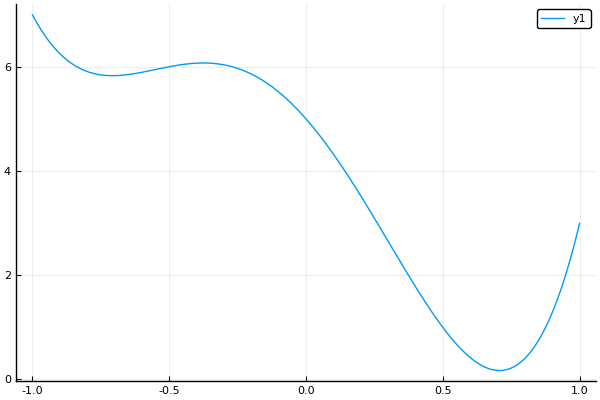
\includegraphics[width=10cm]{poczatkowy.png}
  \centering
  \caption{Wielomian $f(x) = x^4 + x^3 + x^2 + x + 1$ na przedziale $\interval{-1}{1}$}
  \label{fig:wykres1}
\end{figure}
Następnie obliczmy wartości wielomianu w 100 losowych punktach z przedziału $\interval{-1}{1}$ i zaburzmy te wyniki dodając do nich losowe wartości z przedziału $\interval{-\frac{1}{10}}{\frac{1}{10}}$

\begin{figure}[!htbp]
  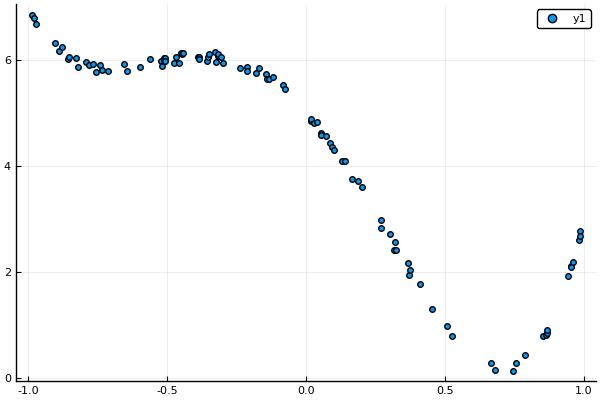
\includegraphics[width=10cm]{zaburzone.png}
  \centering
  \caption{Zaburzone wartości wielomianu}
  \label{fig:wykres2}
\end{figure}

Jest to dokładnie problem opisany we wsętpie - mamy zestaw danych, częściowo zaburzonych. Chcemy jak najlepiej odwzorować pierwotną funkcję.

\subsection{Konstrukcja wielomianów bazowych}
Jak było napisane wcześniej, najlepszym sposobem na rozwiązanie tego problemu jest wcześniejsze wyznaczenie bazy ortogonalnej. Jednak, gdy mamy zbiór skończonej liczby punktów, to nie musimy wyznaczać konkretnego wzoru na $P_i$ a jedynie wyznaczyć wartości w punktach. Pozwoli nam to przy późniejszych obliczeniach wykorzystać już gotowe wartości. Należy także zapamiętać wielkości $c_k$ i $d_k$ - będą potrzebne przy liczeniu wartości wielomianu optymalnego algorytmem Clenshawa.

Żeby wykorzystać trójzależność wielomianów ortogonalnych najlepiej też od razu liczyć wartości współczynników $a_k$, wystarczy wtedy pamiętać trzy wielomiany bazowe zamiast wszystkich.

\subsection{Konstrukcja wielomianów optymalnych}
Jak było powiedziane w poprzednim podrozdziale współczynniki $a_k$, $c_k$ i $d_k$ zostały już policzone. Zostało teraz tylo wyznaczenie wielomianu optymalnego. Ponownie nie musimy wyznaczać ogólnej postaci wielomianu $w_n$ - wystarczy znać jego wartość w punktach, co sprowadza się do wyliczenia za pomocą algorytmu Clenshawa.
W celu prezentacji wykresów wartości $w_n$ zostały obliczone w 1000 równoodległych punktach.

Na wykresie \ref{fig:example} zostało przedstawionych kilka pierwszych wielomianów optymalnych
\begin{figure}%
    \centering
    \subfloat[pierwszy wielomian optymalny]{{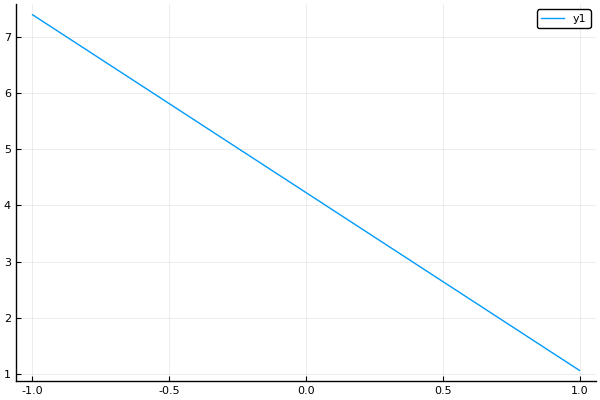
\includegraphics[width=7cm]{opt1.png} }}%
    \qquad
    \subfloat[drugi wielomian optymalny]{{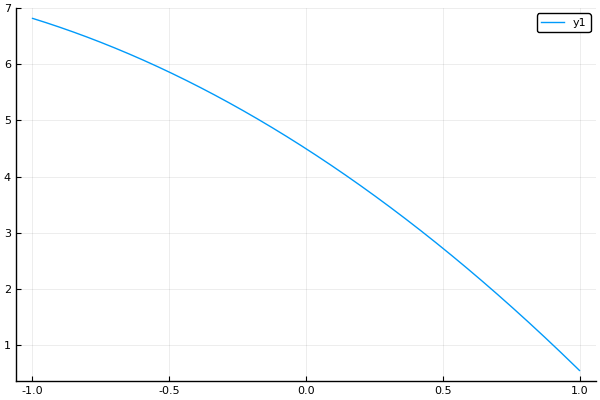
\includegraphics[width=7cm]{opt2.png} }}%
    \qquad
    \subfloat[trzeci wielomian optymalny]{{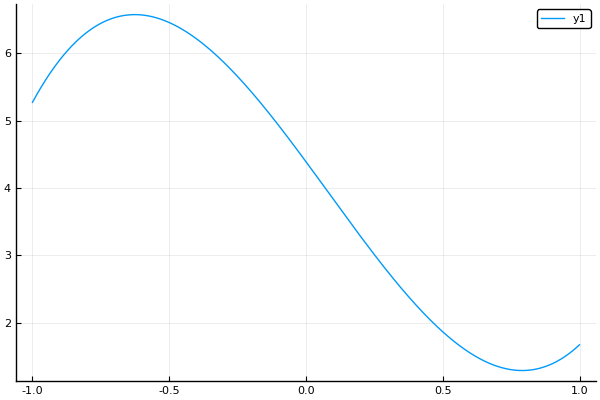
\includegraphics[width=7cm]{opt3.png} }}
    \qquad
    \subfloat[czwarty wielomian optymalny]{{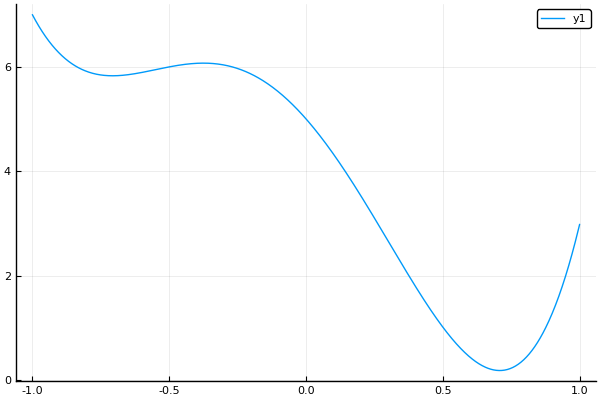
\includegraphics[width=7cm]{opt4.png} }}
    \qquad
    \subfloat[piąty wielomian optymalny]{{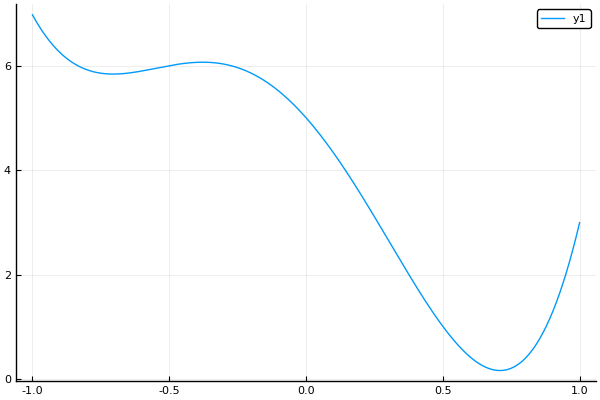
\includegraphics[width=7cm]{opt5.png} }}
    \qquad
    \subfloat[szósty wielomian optymalny]{{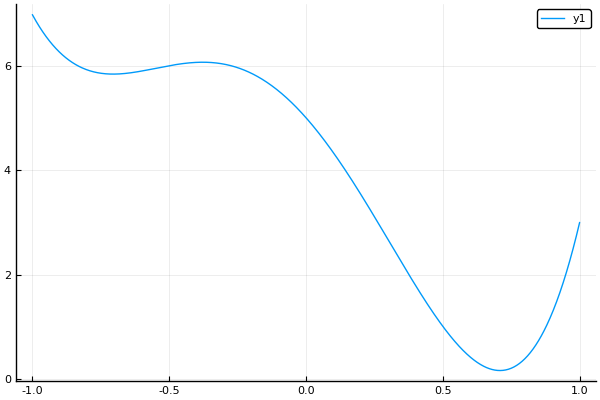
\includegraphics[width=7cm]{opt6.png} }}
    \caption{Wielomiany optymalne}
    \label{fig:example}%
\end{figure}

Widać, że już czwarty wielomian optymalny przypomina wybraną funkcję czwartego stopnia, a piąty i szósty wyglądają podobnie. Wydawałoby się, że czym wyższy stopień, tym wielomian aproksymujący będzie lepszy - nie jest to prawda. Jeżeli spojrzymy na trzydziesty wielomian optymalny na rysunku \ref{fig:wykres4}, to odbiega on znacznie od oryginalnego. Są tego dwie przyczyny. Wylosowane węzły nie są dokładnie wielomianem pierwotnym, więc próbując przybliżyć się do nich możemy oddalać się od oryginalniej funkcji. Co więcej, czym wyższy stopień wielomianu, tym wiecej obliczeń, co prowadzi do kumulacji błędów zaokrągleń. 
\begin{figure}[!htbp]
  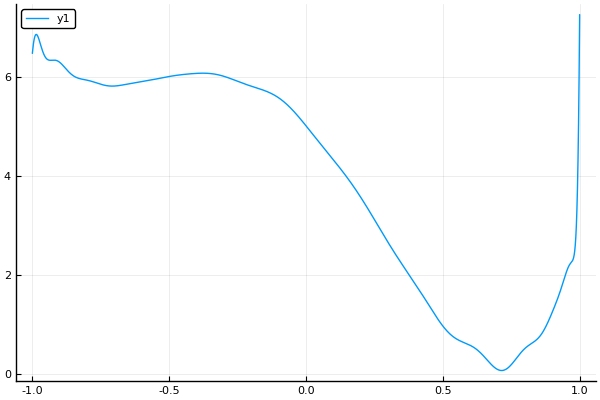
\includegraphics[width=10cm]{opt30.png}
  \centering
  \caption{30-ty wielomian optymalny}
  \label{fig:wykres4}
\end{figure}

Warto zauważyć, że gdy będziemy rozważać 99-ty wielomian optymalny, to będzie to dokładnie interpolacja - mamy 100 punktów i szukamy takiego wielomianu, którego odległość od tych punktów jest jak najmniejsza. Możemy zbudować taki wielomian, który dokładnie przez te punkty przejdzie. Jednak jest on mocno niestabilny - jak widać na wykresie \ref{fig:wykres5} mocno maleje w okolicy -1, przez co ciężko porównać wykres do pierwotnej funkcji. 
\begin{figure}[!htbp]
  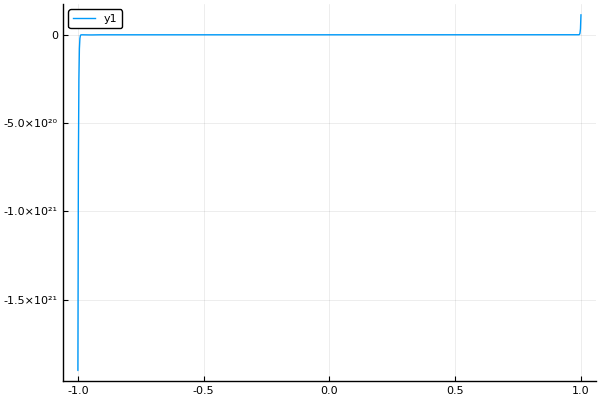
\includegraphics[width=10cm]{opt99.png}
  \centering
  \caption{99-ty wielomian optymalny}
  \label{fig:wykres5}
\end{figure}

Widząc to ciekawe zachowanie wielomianów optymalnych można, przyjrzeć się maksymalnemu odchyleniu we wcześniej losowanych 100 węzłach. Tabela \ref{table:bledy} pokazuje właśnie to maksymalne odchylenie w stosunku do pierwotnych wartości funkcji, jak i tych zaburzonych. Jak widać najmniejsze maksymalne odchylenie jest przy czwartym wielomianie optymalnym (czyli ten sam stopień co oryginalny wielomian). Późniejsze wyniki są już tylko mniej dokładne.
\begin{table}
\begin{center}
\begin{tabular}{ c| c| c }
max stopień &wartości oryginalne & wartości zaburzone \\
\hline
1 & 1.91038405 & 1.92009947 \\
2 & 2.07132017 & 2.14547981 \\
3 & 1.48622452 & 1.48810183 \\
4 & 0.01332262 & 0.10600691 \\
5 & 0.02046311 & 0.11333113 \\
6 & 0.02063537 & 0.11352204 \\
\vdots & \vdots & \vdots \\
30 & 0.10492267 & 0.10629689 \\
\vdots & \vdots & \vdots \\
96 & 15.13903492 & 15.13715761 \\
97 & 47.13903492 & 47.13715761 \\
98 & 25.13903492 & 25.13715761 \\
99 & 15.13903492 & 15.13715761 \\
\end{tabular}
\end{center}
\caption{Tabela błędów (odchyleń) w 100 wcześniej losowanych punktach}
\label{table:bledy}
\end{table}


\section{Uwagi}
Można jeszcze bardziej zaoszczędzić pracy przy liczeniu wielomianów ortogonalnych. Jeśli wybierzemy równoodległe węzły i odpowiednią funkcję wagową to wielomiany ortogonalne są już wyznaczone co pozwala pominąć wszystkie obliczenia z nimi związane. Jednak w przypadku tego zadania punkty są całkowicie losowe, nie można więc z tego ułatwienia skorzystać.
\section{Podsumowanie}
Praktyczna część tego zadania pokazuje, że aproksymacja jest dobrym rozwiązaniem problemu przybliżania zbioru danych funkcją (wielomianem).  Mając nawet wiele punktów możemy przybliżyć je wielomianem o stosunkowo niskim stopniu. Jak widzieliśmy wcześniej zwiększanie stopnia pogarszało nawet wyniki. Pozwala nam to na łatwiejszą analizę danych i opsywanie zjawisk za pomocą funkcji, które są znacznie łatwiejsze w interpretacji niż zbiór danych.

\begin{thebibliography}{9}
\bibitem{kincaid} David Kincaid, Ward Cheney
\emph{Analiza Numeryczna},
Warszawa, WNT, 2006.
\bibitem{jankowscy} Janina i Michał Jankowscy
\emph{Przegląd metod i algorytmów numerycznych},
Warszawa, WNT, 1981.
\bibitem{paper1} Sławomir Milewski
\emph{Metody numeryczne część druga},
Samodzielny Zakład Metod Komputerowych w Mechanice L6, WIL, PK.
\bibitem{metody} Zenon Fortuna, Bohdan Macukow, Janusz Wąsowski
\emph{Metody Numeryczne},
Warszawa, WNT, 2001.
\end{thebibliography}

\end{document}


